
\begin{frame}
  \frametitle{Training Set Size: Learning Curves}
  \begin{figure}[h!]
    \centering
    \begin{minipage}{0.35\textwidth}
      \centering
      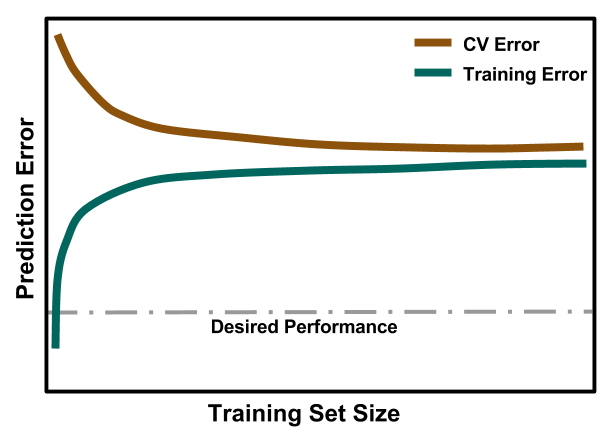
\includegraphics[width=\linewidth]{./figures/LearningCurve-bias.png}
    \end{minipage}%
    \begin{minipage}{0.35\textwidth}
      \centering
      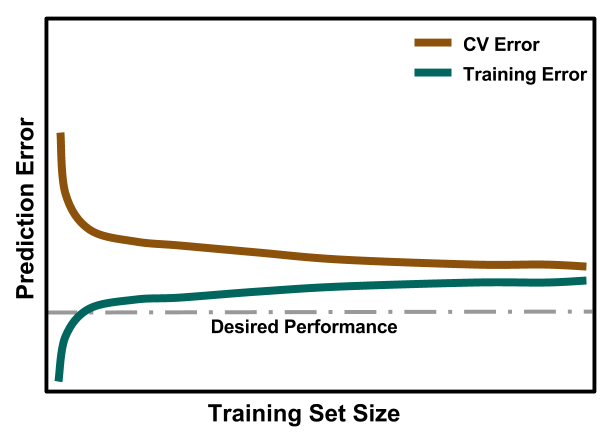
\includegraphics[width=\linewidth]{./figures/LearningCurve-ideal.png}
    \end{minipage}%
    \begin{minipage}{0.35\textwidth}
      \centering
      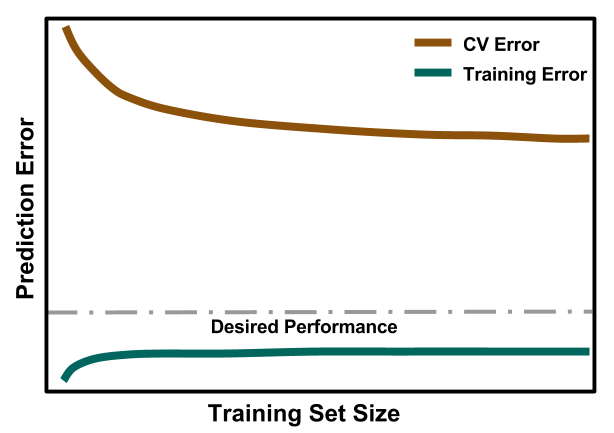
\includegraphics[width=\linewidth]{./figures/LearningCurve-variance.png}
    \end{minipage}
    \caption{Learning curves for three training scenarios: high bias, balanced bias and variance, and high variance}
  \end{figure}
\end{frame}

\begin{frame}
  \frametitle{Model Complexity: Validation Curves}
  \begin{figure}[h!]
    \centering
    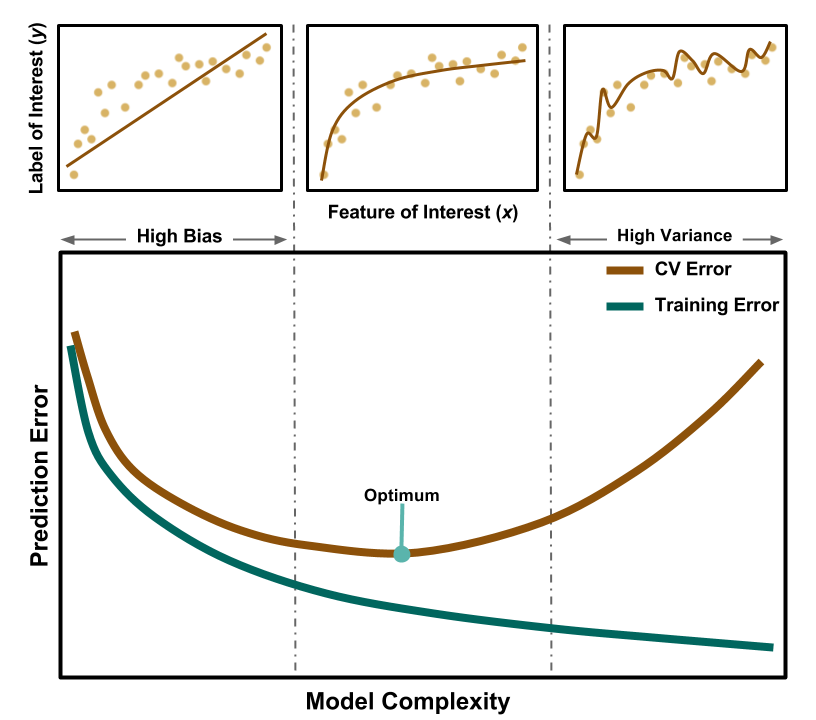
\includegraphics[height=0.7\textheight]{./figures/ValidationCurve.png}
    \caption{Validation curve showing different fitness of models}
  \end{figure}
\end{frame}

\begin{frame}
  \frametitle{Model Comparison}
  \begin{minipage}{0.5\textwidth}
    \centering
    \begin{table}[h!]
      \centering
      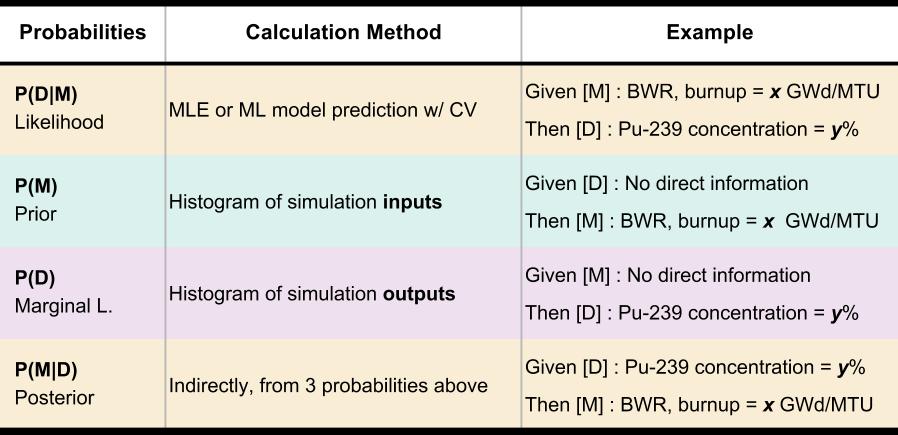
\includegraphics[height=0.7\textheight]{./figures/bayes.png}
      \caption{Bayes}
    \end{table}
  \end{minipage}%
  \begin{minipage}{0.5\textwidth}
    \centering
    \begin{equation}
      Posterior = \frac{Likelihood * Prior}{Marginal \ Likelihood} 
    \end{equation}
  \end{minipage}
\end{frame}

